\documentclass{article}
\usepackage{header} % Required for inserting images
% \newcommand{\p}[1]{$\mathbb{P}(#1)$}


\title{\LARGE{Теория вероятностей и математическая статистика—2}\\
Теоретический и задачный минимумы\\
ФЭН НИУ ВШЭ}
\author{Винер Даниил  \href{https://t.me/danya_vin}{@danya\_vin}}
\date{Версия от \today}

\begin{document}
\maketitle
\begin{flushright}
    \textit{Спасибо Яне Рейтман за эстетик конспект}
\end{flushright}
\tableofcontents
\newpage
\setlength{\parindent}{15pt}
\setlength{\parskip}{2mm}
\setlist[itemize]{left=1cm}
\setlist[enumerate]{left=1cm}
\section{Теоретический минимум}

\subsection{Сформулируйте неравенство Крамера-Рао для несмещённых оценок}
\definition Пусть $X=(X_1,\ldots,X_n)$ — случайная выборка и $\ell(x_1,\ldots,x_m;\theta)$ — логарифмическая функция правдоподобия. Тогда, величина 
\begin{equation*}
    I_n(\theta)=\matwait{\left(\frac{\partial}{\partial\theta}\ell(x_1,\ldots,x_n\theta)\right)^2}
\end{equation*}
называется \textit{информацией Фишера} о параметре $\theta$, содержащейся в $n$ наблюдениях случайной выборки $X$

\theorem Пусть $\widehat{\theta}$ — несмещенная оценка параметра $\theta$, а также выполнены некоторые условия регулярности. Тогда, имеет место неравенство (\textit{Рао-Крамера}):
\begin{equation*}
    I_n^{-1}(\theta)\leqslant \dispersia{\widehat{\theta}}
\end{equation*}

\definition Несмещенная оценка $\widehat{\theta}$ называется \textit{эффективной} оценкой параметра $\theta$, если для нее неравенство Рао-Крамера обращается в равенство
\begin{equation*}
    I_n^{-1}(\theta)= \dispersia{\widehat{\theta}}
\end{equation*} 

\subsection{Дайте определение функции правдоподобия и логарифмической функция правдоподобия}
\definition Пусть задана случайная выборка $X=\left(X_{1}, \ldots, X_{n}\right)$, компоненты которой имеют функцию распределения $F(x; \theta)$, зависящую от неизвестного параметра $\theta \in \Theta$
\begin{itemize}
    \item Если случайный вектор $X=\left(X_{1}, \ldots, X_{n}\right)$ имеет дискретное распределение, то его функцией правдоподобия называется совместная вероятность
    \begin{equation*}
        \mathcal{L}\left(x_{1}, \ldots, x_{n} ; \theta\right):=\mathbb{P}_{\theta}\left(\left\{X_{1}=x_{1}\right\} \cap \ldots \cap\left\{X_{n}=x_{n}\right\}\right),
    \end{equation*}
    которая рассматривается как функция от переменной $\theta$ при фиксированных значениях переменных $x_1,\ldots,x_n$

    \item  Если случайный вектор $X=\left(X_{1}, \ldots, X_{n}\right)$ имеет абсолютно непрерывное распределение, то его функцией правдоподобия называется совместная плотность
    \begin{equation*}
        \mathcal{L}\left(x_{1}, \ldots, x_{n} ; \theta\right):=f_{X_{1}, \ldots, X_{n}}\left(x_{1}, \ldots, x_{n} ; \theta\right)
    \end{equation*}
    В независимом случае:
    \begin{equation*}
        \mathcal{L}\left(x_{1}, \ldots, x_{n} ; \theta\right)=f_{X_{1}}\left(x_{1} ; \theta\right) \cdot \ldots \cdot f_{X_{n}}\left(x_{n} ; \theta\right)
    \end{equation*}
\end{itemize}

\definition Логарифмической функцией правдоподобия называется функция
\begin{equation*}
    l\left(x_{1}, \ldots, x_{n} ; \theta\right):=\ln \mathcal{L}\left(x_{1}, \ldots, x_{n} ; \theta\right)
\end{equation*}

\subsection{Дайте определение информации Фишера о параметре $\theta$, содержащейся в одном наблюдении}
\definition Информацией Фишера за одно наблюдение называется
\begin{equation*}
    \underbrace{I_1(\theta)}_{i(\theta)}=\matwait{\left(\frac{\partial}{\partial\theta}\ell(x_1;\theta)\right)^2}
\end{equation*}

\subsection{Дайте определение оценки метода моментов параметра $\theta$ с использованием первого момента, если $\mathrm{E}\left(X_{i}\right)=g(\theta)$ и существует обратная функция $g^{-1}$}
$\mu_1=\widehat{\mu}_1$ — моментное тождество, где $\mu_1=\matwait{X_i}=g(\theta)$, $\widehat{\mu}_1=\overline{X}$, $g(\theta)=\overline{X}$

$g(\theta)$ имеет обратную функцию $\theta=g^{-1}(\overline{X})$

\definition Оценка метода моментов параметра $\theta$ определяется как:
\begin{equation*}
    \hat{\theta}_{MM} = g^{-1}\left( \overline{X} \right)
\end{equation*}

\subsection{Дайте определение оценки метода максимального правдоподобия параметра $\theta$}
\definition Оценкой $\hat{\theta}_{ML}$ неизвестного параметра $\theta \in \Theta$ по ММП называется точка глобального максимума функции правдоподобия по переменной $\theta \in \Theta$ при фиксированных значениях переменных $x_{1}, \ldots, x_{n}$, т.е.
\begin{equation*}
    \mathcal{L}\left(x_{1}, \ldots, x_{n} ; \hat{\theta}_{ML}\right)=\max _{\theta \in \Theta} \mathcal{L}\left(x_{1}, \ldots, x_{n} ; \theta\right)
\end{equation*}

\subsection{Укажите закон распределения выборочного среднего, величины $\frac{\overline{X}-\mu}{\sigma / \sqrt{n}}$, величины $\frac{\overline{X}-\mu}{\hat{\sigma} / \sqrt{n}}$, величины $\frac{\hat{\sigma}^{2}(n-1)}{\sigma^{2}}$}
Пусть $X_{1}, \ldots, X_{n}$ — независимые случайные величины, $X_i\sim(\mu,\sigma^2)$%, $\overline{X}:=\frac{X_{1}+\ldots+X_{n}}{n}$ - выборочное среднее, а $\widehat{\sigma^{2}}:=\frac{1}{n-1} \sum_{i=1}^{n}\left(X_{i}-\overline{X}\right)^{2}$ исправленная выборочная дисперсия. Тогда
\begin{itemize}
    \item $\frac{\overline{X}-\mu}{\sqrt{\frac{\sigma^2}{n}}}\sim\mathcal{N}(0;1)$
    \item $\frac{\overline{X}-\mu}{\sqrt{\frac{\hat{\sigma}^2}{n}}}\sim t_{n-1}$, $\widehat{\sigma^{2}}:=\frac{1}{n-1} \sum_{i=1}^{n}\left(X_{i}-\overline{X}\right)^{2}$
    \item $\frac{\hat{\sigma}^{2}(n-1)}{\sigma^{2}} \sim \chi^{2}(n-1)$
    \item $\overline{X} \sim \mathcal{N}\left(\mu, \frac{\sigma^2}{n} \right)$, $\overline{X}:=\frac{X_{1}+\ldots+X_{n}}{n}$
\end{itemize}
\subsection{Укажите формулу доверительного интервала с уровнем доверия $(1-\alpha)$ для $\mu$ при известной дисперсии, для $\mu$ при неизвестной дисперсии, для $\sigma^{2}$}
Пусть $X=(X_1,\ldots,X_n)$ — независимые случайные величины, $X_i\sim(\mu,\sigma^2)$
\subsubsection{Для $\mu$ при известной дисперсии}
Доверительный интервал для $\mu$ при известной дисперсии $\sigma^2$ уровня доверия $\gamma=1-\alpha$

$T(\text{статистика})=\displaystyle\frac{\overline{X}-\mu}{\sqrt{\frac{\sigma^2}{n}}}\sim\mathcal{N}(0;1)$
\begin{center}
    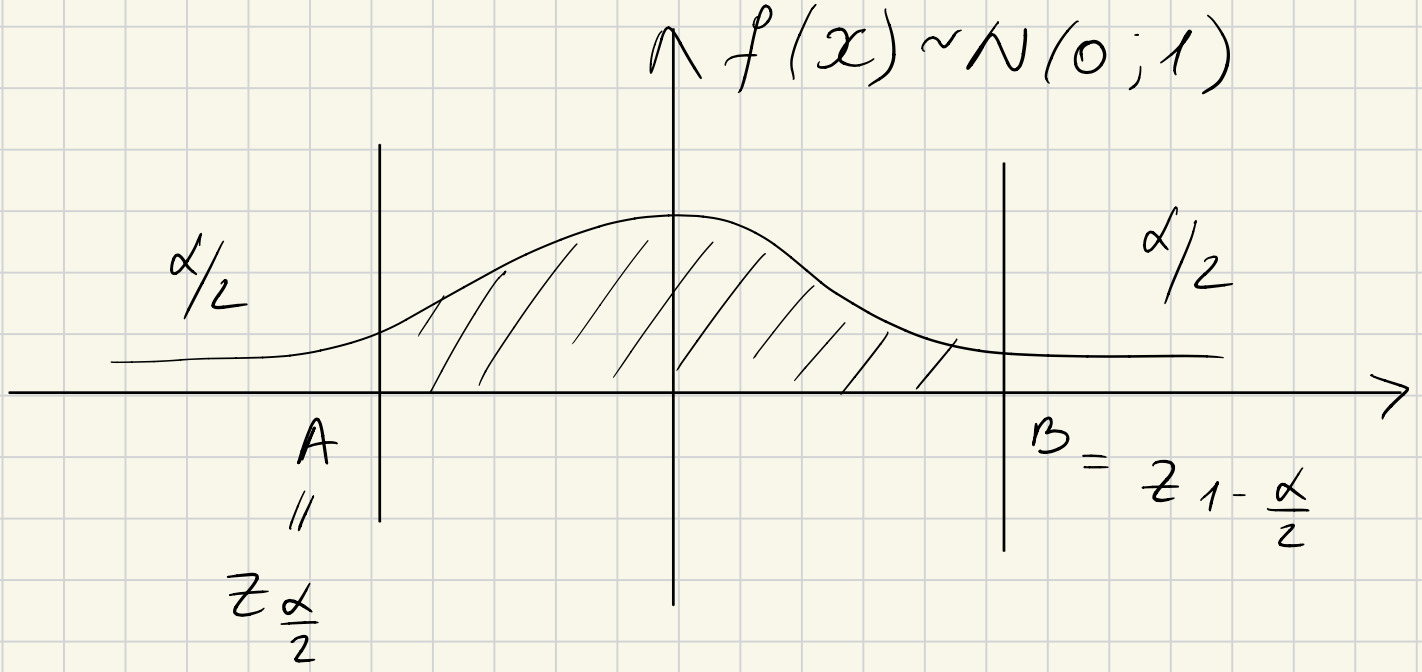
\includegraphics[width=0.5\linewidth]{confidence_interval.png}
\end{center}
С вероятностью $\gamma$ выполняется событие:
\begin{equation*}
    \begin{aligned}
        A\leqslant T\leqslant B&\Longleftrightarrow A\leqslant \frac{\overline{X}-\mu}{\sqrt{\frac{\sigma^2}{n}}}\leqslant B\\
        &\Longleftrightarrow A\sqrt{\frac{\sigma^2}{n}}\leqslant\overline{X}-\mu\leqslant B\sqrt{\frac{\sigma^2}{n}}\\
        &\Longleftrightarrow-\overline{X}+A\sqrt{\frac{\sigma^2}{n}}\leqslant-\mu\leqslant-\overline{X}+B\sqrt{\frac{\sigma^2}{n}}\\
        &\Longleftrightarrow\overline{X}-B\sqrt{\frac{\sigma^2}{n}}\leqslant\mu\leqslant\overline{X}-A\sqrt{\frac{\sigma^2}{n}}\\
        &-z_{\alpha/2}=z_{1-\alpha/2}\\
        &\Longleftrightarrow\overline{X}-z_{1-\alpha/2}\sqrt{\frac{\sigma^2}{n}}\leqslant\mu\leqslant\overline{X}-z_{\alpha/2}\sqrt{\frac{\sigma^2}{n}}\\
        &-z_{1-\alpha/2}=z_{\alpha/2}\\
        &\Longleftrightarrow\underbrace{\overline{X}+z_{\alpha/2}\sqrt{\frac{\sigma^2}{n}}}_{T_1(X)}\leqslant\mu\leqslant\underbrace{\overline{X}+z_{1-\alpha/2}\sqrt{\frac{\sigma^2}{n}}}_{T_2(X)}
    \end{aligned}
\end{equation*}

\subsubsection{Для $\mu$ при неизвестной дисперсии}
Доверительный интервал для $\mu$ при неизвестной дисперсии $\sigma^2$ уровня доверия $\gamma=1-\alpha$

$T=\displaystyle\frac{\overline{X}-\mu}{\sqrt{\frac{\widehat{\sigma}^2}{n}}}\sim t_{n-1}$, где $\widehat{\sigma^{2}}:=\displaystyle\frac{1}{n-1} \sum_{i=1}^{n}\left(X_{i}-\overline{X}\right)^{2}$

\begin{center}
    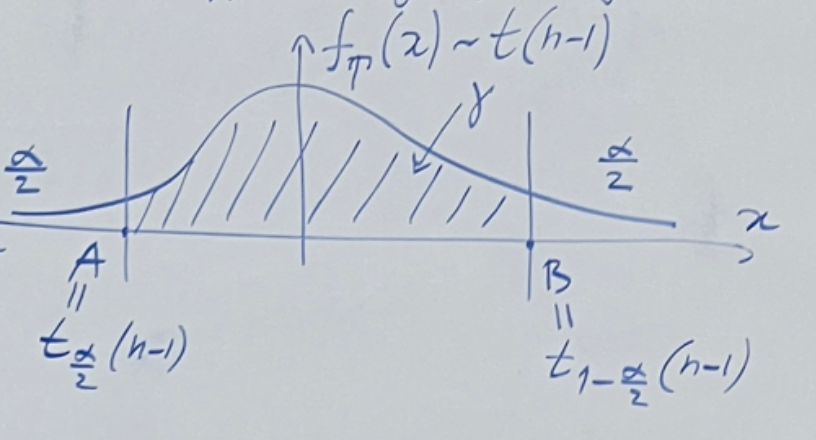
\includegraphics[width=0.5\linewidth]{confidence_interval4.png}
\end{center}
С вероятностью $\gamma$ выполняется событие:
\begin{equation*}
    \begin{aligned}
        A\leqslant T\leqslant B&\Longleftrightarrow A\leqslant \frac{\overline{X}-\mu}{\sqrt{\frac{\widehat{\sigma}^2}{n}}}\leqslant B\\
        &\Longleftrightarrow A\sqrt{\frac{\widehat{\sigma}^2}{n}}\leqslant\overline{X}-\mu\leqslant B\sqrt{\frac{\widehat{\sigma}^2}{n}}\\
        &\Longleftrightarrow-\overline{X}+A\sqrt{\frac{\widehat{\sigma}^2}{n}}\leqslant-\mu\leqslant-\overline{X}+B\sqrt{\frac{\widehat{\sigma}^2}{n}}\\
        &\Longleftrightarrow\overline{X}-B\sqrt{\frac{\widehat{\sigma}^2}{n}}\leqslant\mu\leqslant\overline{X}-A\sqrt{\frac{\widehat{\sigma}^2}{n}}\\
        &\Longleftrightarrow\overline{X}-t_{n-1,1-\alpha/2}\sqrt{\frac{\widehat{\sigma}^2}{n}}\leqslant\mu\leqslant\overline{X}-t_{n-1,\alpha/2}\sqrt{\frac{\widehat{\sigma}^2}{n}}\\
        &\Longleftrightarrow\underbrace{\overline{X}+t_{n-1,\alpha/2}\sqrt{\frac{\widehat{\sigma}^2}{n}}}_{T_1(X)}\leqslant\mu\leqslant\underbrace{\overline{X}+t_{n-1,1-\alpha/2}\sqrt{\frac{\widehat{\sigma}^2}{n}}}_{T_2(X)}
    \end{aligned}
\end{equation*}

\subsubsection{Для $\sigma^2$}
Доверительный интервал для $\sigma^2$ при неизветсном математическом ожидании уровня доверия $\gamma=1-\alpha$

$T=\displaystyle\frac{\widehat{\sigma}^2(n-1)}{\sigma^2}\sim\chi^2(n-1)$

\begin{center}
    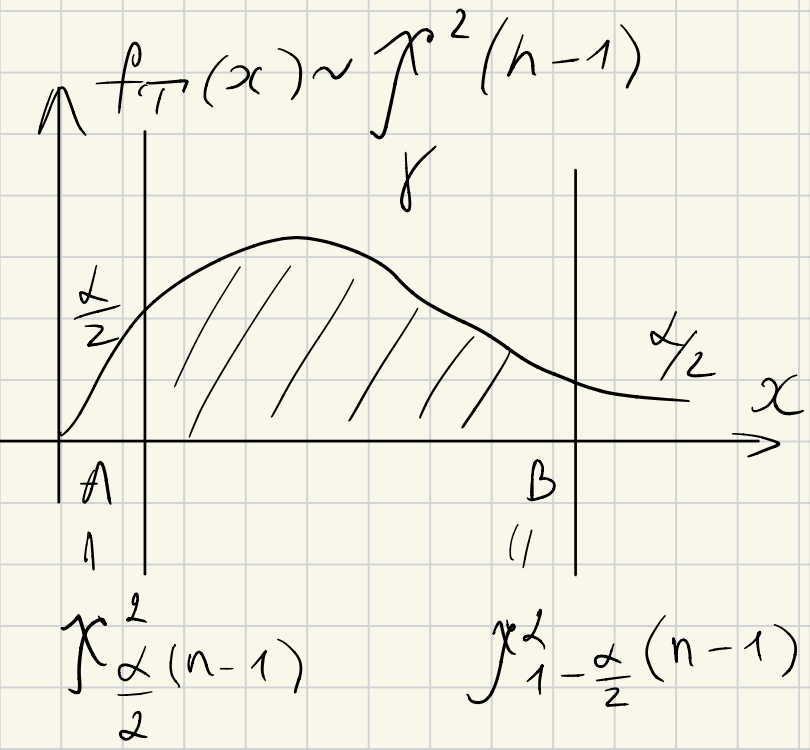
\includegraphics[width=0.5\linewidth]{confidence_interval2.png}
\end{center}
С вероятностью $\gamma$ выполняется событие:
\begin{equation*}
    \begin{aligned}
        A\leqslant T\leqslant B&\Longleftrightarrow A\leqslant \frac{\widehat{\sigma}^2(n-1)}{\sigma^2}\leqslant B\\
        &\Longleftrightarrow \begin{cases}
            A\leqslant\frac{\widehat{\sigma}^2(n-1)}{\sigma^2}\\
            \frac{\widehat{\sigma}^2(n-1)}{\sigma^2}\leqslant B
        \end{cases}\\
        &\Longleftrightarrow\begin{cases}
            \sigma^2\leqslant\frac{\widehat{\sigma}^2(n-1)}{A}\\
            \frac{\widehat{\sigma}^2(n-1)}{B}\leqslant\sigma^2
        \end{cases}\\
        &\Longleftrightarrow\frac{\widehat{\sigma}^2(n-1)}{B}\leqslant\sigma^2\leqslant\frac{\widehat{\sigma}^2(n-1)}{A}\\
        &\Longleftrightarrow\underbrace{\frac{\widehat{\sigma}^2(n-1)}{\chi^2_{1-\alpha/2}(n-1)}}_{T_1(X)}\leqslant\sigma^2\leqslant\underbrace{\frac{\widehat{\sigma}^2(n-1)}{\chi^2_{\alpha/2}(n-1)}}_{T_2(X)}
    \end{aligned}
\end{equation*}

\subsection{Дайте определение ошибки первого и второго рода, критической области}
Пусть $X=(X_1,\ldots,X_n)$ — случайная выборка с плотностью распределения $f_{X_1,\ldots,X_n}(x_1,\ldots,x_n)$

Пусть $f_0(x_1,\ldots,x_n)$ и $f_1(x_1,\ldots,x_n)$ — две конкретные функции плотности, при этом $$f_0(x_1,\ldots,x_n)\ne f_1(x_1,\ldots,x_n)$$

Мы хотим проверить две гипотезы:
\begin{itemize}
    \item $H_0:$ $f_{X_1,\ldots,X_n}(x_1,\ldots,x_n)=f_0(x_1,\ldots,x_n)$
    \item $H_1:$ $f_{X_1,\ldots,X_n}(x_1,\ldots,x_n)=f_1(x_1,\ldots,x_n)$
\end{itemize}
Рассмотрим множество $S\in\mathbb{R}^n$ — критическую область. Тогда, $S$-критерием называется правило
\begin{itemize}
    \item если $(x_1,\ldots,x_n)\in S$, то мы принимаем $H_1$
    \item если $(x_1,\ldots,x_n)\not\in S$, то мы принимаем $H_0$
\end{itemize}

При этом, возможны такие 4 ситуации:
\begin{center}
    \begin{tabular}{c|c|c}
        &accepted $H_0$&accepted $H_1$\\
        \hline
        real $H_0$&OK&ошибка 1 рода\\
        \hline
        real $H_1$&ошибка 2 рода&OK
    \end{tabular}
\end{center}

\subsection{Укажите формулу доверительного интервала с уровнем доверия $(1-\alpha)$ для вероятности успеха, построенного по случайной выборке большого размера из распределения Бернулли $\operatorname{Be}(p)$}
Дана выборка $X_1,\ldots,X_n$ — независимые случайные величины, $X_i\sim Be(p)$, $p\in(0;1)$

Доверительный интервал для $p$ уровня доверия $\gamma=1-\alpha$

$T=\displaystyle\frac{\overline{X}-p}{\sqrt{\frac{\overline{X}(1-\overline{X})}{n}}}\sim \mathcal{N}(0;1)$

\begin{center}
    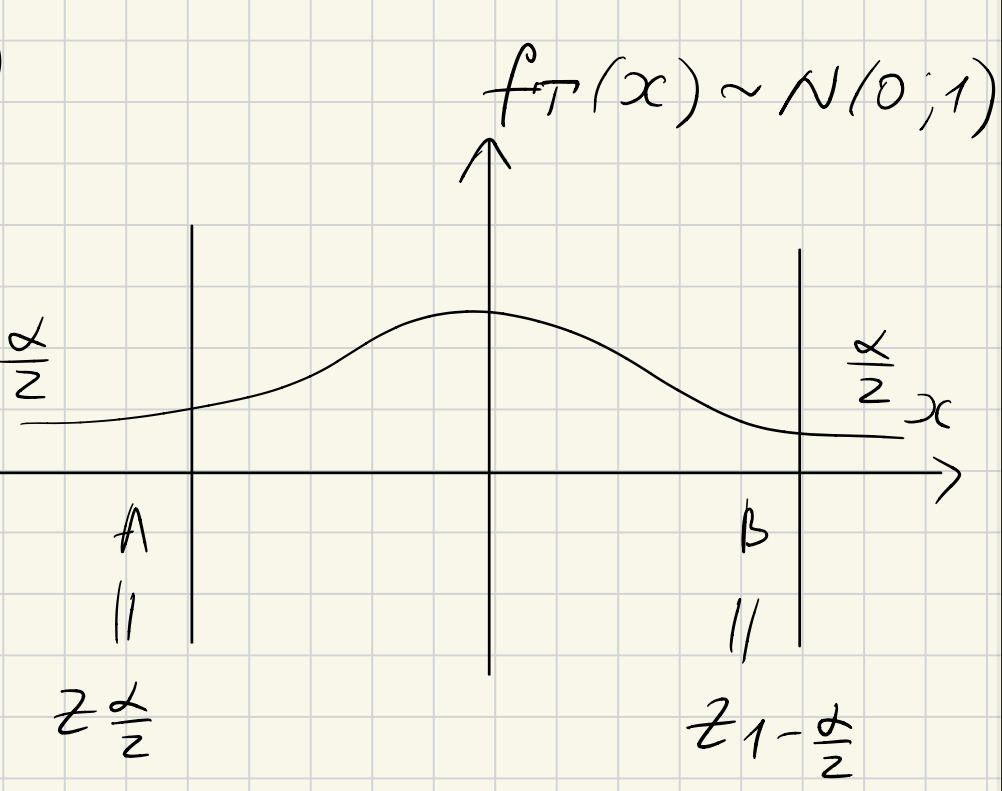
\includegraphics[width=0.5\linewidth]{confidence_interval3.png}
\end{center}
С вероятностью $\gamma$ выполняется событие:
\begin{equation*}
    \begin{aligned}
        A\leqslant p\leqslant B&\Longleftrightarrow A\leqslant \frac{\overline{X}-p}{\sqrt{\frac{\overline{X}(1-\overline{X})}{n}}}\leqslant B\\
        &\Longleftrightarrow A\sqrt{\frac{\overline{X}(1-\overline{X})}{n}}\leqslant \overline{X}-p\leqslant B\sqrt{\frac{\overline{X}(1-\overline{X})}{n}}\\
        &\Longleftrightarrow-\overline{X}+A\sqrt{\frac{\overline{X}(1-\overline{X})}{n}}\leqslant-p\leqslant-\overline{X}+B\sqrt{\frac{\overline{X}(1-\overline{X})}{n}}\\
        &\Longleftrightarrow\overline{X}-A\sqrt{\frac{\overline{X}(1-\overline{X})}{n}}\leqslant p\leqslant\overline{X}-B\sqrt{\frac{\overline{X}(1-\overline{X})}{n}}\\
        &\Longleftrightarrow\overline{X}-z_{\alpha/2}\sqrt{\frac{\overline{X}(1-\overline{X})}{n}}\leqslant p\leqslant\overline{X}-z_{1-\alpha/2}\sqrt{\frac{\overline{X}(1-\overline{X})}{n}}
    \end{aligned}
\end{equation*}

\newpage
\section{Задачный минимум}
\subsection{Пусть$ X_1, \ldots, X_n$ — случайная выборка из распределения с плотностью распределения...}
\begin{equation*}
    f(x, \theta)= \begin{cases}\frac{6 x(\theta-x)}{\theta^{3}} & \text { при } x \in[0 ; \theta] \\ 0 & \text { при } x \notin[0 ; \theta]\end{cases}
\end{equation*}
где $\theta>0$ — неизвестный параметр распределения. Используя центральный момент второго порядка, при помощи метода моментов найдите оценку для неизвестного параметра $\theta$.

Составим моментное тождество $\nu_2=\widehat{\nu}_2$. Найдем $\nu_2$:
\begin{equation*}
    \begin{aligned}
        \nu_2=\matwait{(X_i-\matwait{X_i})^2}=\dispersia{X_i}&=\matwait{X_i^2}-(\matwait{X_i})^2\\
        &=\frac{3\theta^2}{10}-\frac{\theta^2}{4}\\
        &=\frac{\theta^2}{20}
    \end{aligned}
\end{equation*}
При этом, $\widehat{\nu}_2=\frac{1}{n}\sum_{i=1}^{n}(X_i-\overline{X})^2$, тогда моментное тождество $\nu_2=\widehat{\nu}_2$ принимает вид
\begin{equation*}
    \frac{\theta^2}{20}=\frac{1}{n}\sum_{i=1}^{n}(X_i-\overline{X})^2\Longrightarrow\widehat{\theta}_{MM}=\sqrt{\frac{20}{n}\sum_{i=1}^n(X_i-\overline{X})^2}
\end{equation*}

% Покажем, что $\frac{1}{n}\sum_{i=1}^{n}(X_i-\overline{X})^2\underset{n\to\infty}{\longrightarrow}\dispersia{X_i}$:
% \begin{equation*}
%     \begin{aligned}
%         \frac{1}{n}\sum_{i=1}^{n}(X_i-\overline{X})^2&=\frac{1}{n}\sum_{i=1}^n(X_i^2-2X_i\overline{X}+\overline{X}^2)\\
%         &=\frac{1}{n}\sum_{i=1}^nX_i^2-\frac{2\overline{X}}{n}\sum_{i=1}^nX_i+\frac{1}{n}\sum_{i=1}^n\overline{X}^2\\
%         &=\frac{1}{n}\sum_{i=1}^nX_i^2-\frac{2\overline{X}}{n}\cdot n\overline{X}+\frac{1}{n}\cdot n\overline{X}^2\\
%         &=\frac{1}{n}\sum_{i=1}^nX_i^2-\overline{X}^2\underset{n\to\infty}{\longrightarrow}\matwait{X_i^2}-(\matwait{X_i})^2=\dispersia{X_i}
%     \end{aligned}
% \end{equation*}

% Тогда, учитывая, что $\theta>0$, получается, что
% \begin{equation*}
%     \widehat{\theta}_{MM}=\sqrt{\frac{20}{n}\sum_{i=1}^n(X_i-\overline{X})^2}\underset{n\to\infty}{\longrightarrow}\sqrt{20\cdot\dispersia{X_i}}=\sqrt{20\cdot\frac{\theta^2}{20}}=\theta
% \end{equation*}
% Значит, оценка состоятельна

\subsection{Пусть $X_{1}, \ldots, X_{n}$ — случайная выборка. Случайные величины $X_{1}, \ldots, X_{n}$ имеют дискретное распределение, которое задано при помощи таблицы}
\begin{center}
    \begin{tabular}{cccc}
        \hline$x$ & $-3$ & $0$ & $2$ \\
        \hline $\mathbb{P}\left(X_{i}=x\right)$ & $2 / 3-\theta$ & $1 / 3$ & $\theta$ \\
        \hline
    \end{tabular}
\end{center}

Используя второй начальный момент, при помощи метода моментов найдите оценку неизвестного параметра $\theta$. Для реализации случайной выборки $x=(0,0,-3,0,2)$ найдите числовое значение найденной оценки параметра $\theta$.

По определению метода моментов:
\begin{equation*}
    \matwait{X_i^k}=\mu_k=\widehat{\mu}_k=\frac{1}{n}\sum_{i=1}^nX_i^k,
\end{equation*}
то есть теоретический момент равен выборочному. Найдем $\mu_2=\matwait{X_i^2}:$
\begin{equation*}
    \begin{aligned}
        \matwait{X_i^2}&=(-3)^2\cdot\left(\frac{2}{3}-\theta\right)+0^2\cdot\frac{1}{3}+2^2\cdot\theta\\
        &=6-5\theta
    \end{aligned}
\end{equation*}
Тогда,
\begin{equation*}
    \begin{aligned}
        \mu_2&=\widehat{\mu}_2\\
        6-5\theta&=\frac{1}{n}\sum_{i=1}^nX_i^k\Longrightarrow\theta=\frac{1}{5}\left(6-\frac{1}{n}\sum_{i=1}^nX_i^k\right)
    \end{aligned}
\end{equation*}
Вычислим $\widehat{\mu}_2$:
\begin{equation*}
    \begin{aligned}
        \widehat{\mu}_2&=\frac{1}{n}\sum_{i=1}^nX_i^k\\
        &=\frac{1}{5}\left(0^2+0^2+(-3)^2+0^2+2^2\right)\\
        &=2.6
    \end{aligned}
\end{equation*}
Тогда, численно $\theta=\displaystyle\frac{1}{5}\left(6-\frac{1}{n}\sum_{i=1}^nX_i^k\right)=\frac{1}{5}\left(6-2.6\right)=\frac{1}{5}\cdot3.4=0.68$

\subsection{Пусть $X_{1}, \ldots, X_{n}$ — случайная выборка из распределения с функцией плотности}
\begin{equation*}
    f(x, \theta)= \begin{cases}\frac{2 x}{\theta} e^{-\frac{x^{2}}{\theta}} & \text { при } x>0 \\ 0 & \text { при } x \leqslant 0\end{cases}
\end{equation*}
где $\theta>0$. При помощи метода максимального правдоподобия найдите оценку неизвестного параметра $\theta$

Функция правдоподобия имеет вид
\begin{equation*}
    \begin{aligned}
        \mathcal{L}(x_1,\ldots,x_n;\theta)&=\prod_{i=1}^{n}f_{X_i}(x_i;\theta)\\
        &=\frac{2^n}{\theta^n}\prod_{i=1}^{n}x_i\cdot\exp\left(-\frac{x_i^2}{\theta}\right)
    \end{aligned}
\end{equation*}
Логарифмическая функция правдоподобия:
\begin{equation*}
    \begin{aligned}
        \ell(x_1,\ldots,x_n;\theta)&=n\ln\frac{2}{\theta}+\sum_{i=1}^n\ln\left(x_i\cdot\exp\left(-\frac{x_i^2}{\theta}\right)\right)\\
        &=n\ln\frac{2}{\theta}+\sum_{i=1}^n\ln x_i+\sum_{i=1}^n\ln \exp\left(-\frac{x_i^2}{\theta}\right)\\
        &=n\ln\frac{2}{\theta}+\sum_{i=1}^n\ln x_i-\frac{1}{\theta}\sum_{i=1}^nx_i^2\\
        &=n\ln2-n\ln\theta+\sum_{i=1}^n\ln x_i-\frac{1}{\theta}\sum_{i=1}^nx_i^2
    \end{aligned}
\end{equation*}
Дифференцируем по $\theta$, приравняем к 0 и максимизируем
\begin{equation*}
    \begin{aligned}
        \frac{\partial\ell}{\partial\theta}=-\frac{n}{\theta}+\frac{1}{\theta^2}\sum_{i=1}^nx_i^2&=0\\
        \frac{1}{\theta^2}\sum_{i=1}^nx_i^2&=\frac{n}{\theta}\\
        \sum_{i=1}^nx_i^2&=n\theta\Longrightarrow\widehat{\theta}_{ML}=\frac{1}{n}\sum_{i=1}^nx_i^2
    \end{aligned}
\end{equation*}

\subsection{Пусть $X_{1}, \ldots, X_{n}$ — случайная выборка из распределения Бернулли с параметром $p \in(0 ; 1)$. При помощи метода максимального правдоподобия найдите оценку неизвестного параметра $p$}
Функцию вероятности для величины из распределения Бернулли можно записать так:
\begin{equation*}
    \mathbb{P}\left(X_i,p\right)=p^{X_i}(1-p)^{1-X_i},
\end{equation*}
где $X_i\in\{0,1\}$

Тогда функция правдоподобия имеет вид
\begin{equation*}
    \begin{aligned}
        \mathcal{L}(X_1,\ldots,X_n;p)&=\prod_{i=1}^{n}\mathbb{P}(X_i,p)\\
        &=p^{\textstyle \sum X_i}\cdot(1-p)^{n-\sum X_i}
    \end{aligned}
\end{equation*}
Тогда Логарифмическая функция правдоподобия:
\begin{equation*}
    \ell(X_1,\ldots,X_n;p)=\left(\sum_{i=1}^n X_i\right)\ln p+\left(n-\sum_{i=1}^nX_i\right)\ln(1-p)
\end{equation*}
Дифференцируем по $p$, приравняем к 0 и максимизируем
\begin{equation*}
    \begin{aligned}
        \frac{\partial \ell}{\partial p}=\frac{1}{p}\left(\sum_{i=1}^n X_i\right)-\frac{1}{1-p}\left(n-\sum_{i=1}^n X_i\right)=0
    \end{aligned}
\end{equation*}
Найдем оценку параметра:
\begin{equation*}
    \begin{aligned}
        \frac{1}{p}\left(\sum_{i=1}^n X_i\right)&=\frac{1}{1-p}\left(n-\sum_{i=1}^n X_i\right)\\
        \sum_{i=1}^n X_i(1-p)&=\left(n-\sum_{i=1}^n X_i\right)p\\
        \sum_{i=1}^n X_i-p\sum_{i=1}^n X_i&=np-p\sum_{i=1}^n X_i\\
        \sum_{i=1}^n X_i&=np\Longrightarrow p=\frac{1}{n}\sum_{i=1}^n X_i
    \end{aligned}
\end{equation*}

\subsection{Пусть $X=\left(X_{1}, \ldots, X_{n}\right)$ — случайная выборка из распределения с плотностью}
\begin{equation*}
    f(x, \theta)= \begin{cases}\frac{1}{\theta} e^{-\frac{x}{\theta}} & \text { при } x \geqslant 0 \\ 0 & \text { при } x<0\end{cases}
\end{equation*}
где $\theta>0$ — неизвестный параметр. Является ли оценка $\hat{\theta}=\overline{X}$ эффективной?

Плотность указывает, что у нас экспоненциальное распределение с параметром $\lambda=\frac{1}{\theta}$. Проверим несмещенность оценки
\begin{equation*}
    \begin{aligned}
        \matwait{\widehat{\theta}}&=\matwait{\overline{X}}\\
        &=\matwait{\frac{1}{n}\sum_{i=1}^nX_i}\\
        &=\matwait{X_i}\\
        &=\theta
    \end{aligned}
\end{equation*}
Значит, оценка несмещенная

Теперь найдем информацию Фишера для одного наблюдения, которая определяется как
\begin{equation*}
    I(\theta)=\matwait{\left(\frac{\partial}{\partial\theta}\ln f(x,\theta)\right)^2}
\end{equation*}
Составим функцию правдоподобия
\begin{equation*}
    \ln f(x,\theta)=-\ln\theta-\frac{x}{\theta}\Longrightarrow\frac{\partial}{\partial\theta}\ln f(x,\theta)=-\frac{1}{\theta}+\frac{x}{\theta^2}
\end{equation*}
Тогда,
\begin{equation*}
    \begin{aligned}
        I(\theta)&=\matwait{\left(\frac{\partial}{\partial\theta}\ln f(x,\theta)\right)^2}\\
        &=\matwait{\left(-\frac{1}{\theta}+\frac{x}{\theta^2}\right)^2}\\
        &=\matwait{\frac{1}{\theta^2}-\frac{2x}{\theta^3}+\frac{x^2}{\theta^4}}\\
        &=\frac{1}{\theta^2}-\frac{2}{\theta^3}\matwait{X}+\frac{1}{\theta^4}\matwait{X^2}
    \end{aligned}
\end{equation*}
Вычислим $\matwait{X^2}=\dispersia{X}+(\matwait{X})^2=\left(\frac{1}{\theta}\right)^{-2}+\theta^2=2\theta^2$, тогда
\begin{equation*}
    I(\theta)=\frac{1}{\theta^2}-\frac{2}{\theta^3}\theta+\frac{1}{\theta^4}2\theta^2=\frac{1}{\theta^2}
\end{equation*}

Используем неравенство Рао-Крамера:
\begin{equation*}
    \begin{aligned}
        \dispersia{\widehat{\theta}}&\geqslant\frac{1}{n\cdot I(\theta)}\\
        \dispersia{\overline{X}}&\geqslant\frac{1}{n\cdot\frac{1}{\theta^2}}\\
        \frac{1}{n}\dispersia{X_i}&\geqslant\frac{\theta^2}{n}\\
        \frac{\theta^2}{n}&\geqslant\frac{\theta^2}{n}
    \end{aligned}
\end{equation*}
Неравенство выполняется, значит оценка эффективна

\subsection{[DELETE] Стоимость выборочного исследования генеральной совокупности, состоящей из трех страт,..}
определяется по формуле $T C=c_{1} n_{1}+c_{2} n_{2}+c_{3} n_{3}$, где $c_{i}$ — цена одного наблюдения в $i$-й страте, а $n_{i}$ — число наблюдений, которые приходятся на $i$-ю страту. Найдите $n_{1}, n_{2}$ и $n_{3}$, при которых дисперсия стратифицированного среднего достигает наименьшего значения, если бюджет исследования 8000 и имеется следующая информация:
\begin{center}
    \begin{tabular}{cccc}
        \hline Страта & 1 & 2 & 3 \\
        \hline Среднее значение & 30 & 40 & 50 \\
        Стандартная ошибка & 5 & 10 & 20 \\
        Вес & $25 \%$ & $25 \%$ & $50 \%$ \\
        Цена наблюдения & 1 & 5 & 10 \\
        \hline
    \end{tabular}    
\end{center}

\subsection{Пусть $X_{1}, \ldots, X_{n}$ — случайная выборка из нормального распределения с параметрами $\mu$ и $\sigma^{2}=4$}
Используя реализацию случайной выборки,
\begin{equation*}
    x_{1}=-1.11,\ x_{2}=-6.10,\ x_{3}=2.42
\end{equation*}
постройте $90 \%$-й доверительный интервал для неизвестного параметра $\mu$

Уровень доверия — $0.9=1-\alpha\Longrightarrow\alpha=0.1$ — уровень значимости. Для выборки из нормального распределения с \textbf{известной} дисперсией доверительный интревал имеет вид:
\begin{equation*}
    \overline{X}-z_{1-\alpha/2}\cdot\frac{\sigma}{\sqrt{n}}<\mu<\overline{X}+z_{1-\alpha/2}\cdot\frac{\sigma}{\sqrt{n}},
\end{equation*}
где $z_{1-\alpha/2}$ — квантиль уровня $1-\alpha/2$ для стандратного нормального распределения (из таблички)

\comment $\overline{X}=\displaystyle\frac{-1.11+(-6.10)+2.42}{3}=-\frac{4.79}{3}$

Тогда, в нашем случае:
\begin{equation*}
    \begin{aligned}
        \overline{X}-z_{0.95}\cdot\frac{2}{\sqrt{3}}&<\mu<\overline{X}+z_{0.95}\cdot\frac{2}{\sqrt{3}}\\
        -\frac{4.79}{3}-1.65\cdot\frac{2}{\sqrt{3}}&<\mu<-\frac{4.79}{3}+1.65\cdot\frac{2}{\sqrt{3}}\\
        -3.50192&<\mu<0.30859
    \end{aligned}
\end{equation*}

\subsection{Пусть $X_{1}, \ldots, X_{n}$ — случайная выборка из нормального распределения с неизвестными параметрами $\mu$ и $\sigma^{2}$}
Используя реализацию случайной выборки,
\begin{equation*}
    x_{1}=-1.11,\ x_{2}=-6.10,\ x_{3}=2.42
\end{equation*}
постройте $90 \%$-й доверительный интервал для неизвестного параметра $\mu$

Уровень доверия — $0.9=1-\alpha\Longrightarrow\alpha=0.1$ — уровень значимости. Для выборки из нормального распределения с \textbf{неизвестной} дисперсией доверительный интревал имеет вид:
\begin{equation*}
    \overline{X}-t_{n-1,1-\alpha/2}\cdot\frac{\widehat{\sigma}}{\sqrt{n}}<\mu<\overline{X}+t_{n-1,1-\alpha/2}\cdot\frac{\widehat{\sigma}}{\sqrt{n}}
\end{equation*}
Найдем несмещенную выборочную дисперсию
\begin{equation*}
    \begin{aligned}
        \overline{X}&=\displaystyle\frac{-1.11+(-6.10)+2.42}{3}=-\frac{4.79}{3}\\
        \widehat{\sigma}^2&=\frac{1}{n-1}\sum_{i=1}^n\left(X_i-\overline{X}\right)^2\approx18.32523
    \end{aligned}
\end{equation*}
Тогда, для нашей выборки:
\begin{equation*}
    \begin{aligned}
        -\frac{4.79}{3}-t_{2,0.95}\cdot\frac{\sqrt{\widehat{\sigma}^2}}{\sqrt{3}}&<\mu<-\frac{4.79}{3}+t_{2,0.95}\cdot\frac{\sqrt{\widehat{\sigma}^2}}{\sqrt{3}}\\
        -\frac{4.79}{3}-2.92\cdot\frac{4.2808}{\sqrt{3}}&<\mu<-\frac{4.79}{3}+2.92\cdot\frac{4.2808}{\sqrt{3}}\\
        -8.81351&<\mu<5.62017
    \end{aligned}
\end{equation*}

\subsection{Пусть $X_{1}, \ldots, X_{n}$ — случайная выборка из нормального распределения с неизвестными параметрами $\mu$ и $\sigma^{2}$}
Используя реализацию случайной выборки,
\begin{equation*}
    x_{1}=1.07,\ x_{2}=3.66,\ x_{3}=-4.51
\end{equation*}
постройте $80 \%$-й доверительный интервал для неизвестного параметра $\sigma^{2}$

Уровень доверия — $0.8=1-\alpha\Longrightarrow\alpha=0.2$ — уровень значимости. Для выборки из нормального распределения доверительный интревал имеет вид:
\begin{equation*}
    \frac{(n - 1)\hat{\sigma}^2}{\chi^2_{n-1,1 - \alpha/2}}<\sigma^2< \frac{(n - 1)\hat{\sigma}^2}{\chi^2_{n-1,\alpha/2}},
\end{equation*}
где $\chi^2_{\alpha/2}$, $\chi^2_{1 - \alpha/2}$ — квантили хи-квадрат распределения с $n - 1$ степенями свободы.

Вычислим несмещенную выборочную дисперсию:
\begin{equation*}
    \begin{aligned}
        \overline{X}&=\frac{1.07+3.66-4.51}{3}=\frac{11}{150}\\
        \widehat{\sigma}^2&=\frac{1}{n-1}\sum_{i=1}^n\left(X_i-\overline{X}\right)^2\approx17.43223
    \end{aligned}
\end{equation*}
Тогда, для нашей выборки
\begin{equation*}
    \begin{aligned}
        \frac{2\cdot17.43223}{\chi^2_{2,0.9}}&<\sigma^2<\frac{2\cdot17.43223}{\chi^2_{2,0.1}}\\
        \frac{2\cdot17.43223}{4.605}&<\sigma^2<\frac{2\cdot17.43223}{0.211}\\
        7.571&<\sigma^2<165.23441
    \end{aligned}
\end{equation*}

\subsection{Пусть $X_{1}, \ldots, X_{n}$ и $Y_{1}, \ldots, Y_{m}$ — независимые случайные выборки из нормального распределения с параметрами $(\mu_{X}, \sigma_{X}^{2})$ и $(\mu_{Y}, \sigma_{Y}^{2})$ соответственно, причем $\sigma_{X}^{2}=2$ и $\sigma_{Y}^{2}=1$}

Используя реализации случайных выборок
\begin{equation*}
    \begin{array}{ll}
        x_{1}=-1.11, & x_{2}=-6.10, \quad x_{3}=2.42 \\
        y_{1}=-2.29, & y_{2}=-2.91
        \end{array}
\end{equation*}

постройте $95 \%$-й доверительный интервал для разности математических ожиданий $\mu_{X}-\mu_{Y}$

Уровень доверия — $0.95=1-\alpha\Longrightarrow\alpha=0.05$ — уровень значимости%. Для выборки из нормального распределения с известными дисперсиями доверительный интревал имеет вид:

Требуется найти такие две функции $T_{1}(X, Y)$ и $T_{2}(X, Y)$ от случайных выборок $X$ и $Y$, что
\begin{equation*}
    \forall \mu_{X} \in \mathbb{R},\ \forall \mu_{Y} \in \mathbb{R}: \quad \mathbb{P}\left(\left\{T_{1}(X, Y) \leqslant \mu_{X}-\mu_{Y} \leqslant T_{2}(X, Y)\right\}\right)=\alpha
\end{equation*}
То есть, нужно найти такой интервал $\left[T_{1}(X, Y) ; T_{2}(X, Y)\right]$, который с заданным уровнем доверия (надежности) $\alpha=0.95$ накрывает разность математических ожиданий $\mu_{X}-\mu_{Y}$ при любых возможных значениях параметров $\mu_{X}$ и $\mu_{Y}$

Известно, что
$$
T=\frac{\bar{X}-\bar{Y}-\left(\mu_{X}-\mu_{Y}\right)}{\sqrt{\frac{\sigma_{X}^{2}}{n}+\frac{\sigma_{Y}^{2}}{m}}} \sim N(0,1) .
$$

Обозначим через $z_{\alpha / 2}$ и $z_{1-\alpha / 2}$ квантили стандартного нормального распределения уровней $\alpha / 2$ и $1-\alpha / 2$ соответственно. Тогда $\mathbb{P}\left(\left\{z_{\alpha / 2} \leqslant T \leqslant z_{1-\alpha / 2}\right\}\right)=\alpha$

Далее, имеем
\begin{equation*}
    \begin{aligned}
        z_{\alpha / 2} \leqslant T \leqslant z_{1-\alpha / 2}&\Longleftrightarrow z_{\alpha / 2} \leqslant \frac{\bar{X}-\bar{Y}-\left(\mu_{X}-\mu_{Y}\right)}{\sqrt{\frac{\sigma_{X}^{2}}{n}+\frac{\sigma_{Y}^{2}}{m}}} \leqslant z_{1-\alpha / 2}\\
        &\Longleftrightarrow z_{\alpha / 2} \sqrt{\frac{\sigma_{X}^{2}}{n}+\frac{\sigma_{Y}^{2}}{m}} \leqslant \bar{X}-\bar{Y}-\left(\mu_{X}-\mu_{Y}\right) \leqslant z_{1-\alpha / 2} \sqrt{\frac{\sigma_{X}^{2}}{n}+\frac{\sigma_{Y}^{2}}{m}}\\
        &\Longleftrightarrow -(\bar{X}-\bar{Y})+z_{\alpha / 2} \sqrt{\frac{\sigma_{X}^{2}}{n}+\frac{\sigma_{Y}^{2}}{m}} \leqslant-\left(\mu_{X}-\mu_{Y}\right) \leqslant-(\bar{X}-\bar{Y})+z_{1-\alpha / 2} \sqrt{\frac{\sigma_{X}^{2}}{n}+\frac{\sigma_{Y}^{2}}{m}}\\
        &\Longleftrightarrow \bar{X}-\bar{Y}-z_{1-\alpha / 2} \sqrt{\frac{\sigma_{X}^{2}}{n}+\frac{\sigma_{Y}^{2}}{m}} \leqslant \mu_{X}-\mu_{Y} \leqslant \bar{X}-\bar{Y}-z_{\alpha / 2} \sqrt{\frac{\sigma_{X}^{2}}{n}+\frac{\sigma_{Y}^{2}}{m}}
    \end{aligned}
\end{equation*}

Следовательно, вероятности событий $\left\{z_{\alpha / 2} \leqslant T \leqslant z_{1-\alpha / 2}\right\}$ и $$\left\{\bar{X}-\bar{Y}-z_{1-\alpha / 2} \sqrt{\frac{\sigma_{X}^{2}}{n}+\frac{\sigma_{Y}^{2}}{m}} \leqslant \mu_{X}-\mu_{Y} \leqslant \bar{X}-\bar{Y}-z_{\alpha / 2} \sqrt{\frac{\sigma_{X}^{2}}{n}+\frac{\sigma_{Y}^{2}}{m}}\right\}$$ совпадают и равны $\alpha=0.95$, а значит, $\left[\bar{X}-\bar{Y}-z_{1-\alpha / 2} \sqrt{\frac{\sigma_{X}^{2}}{n}+\frac{\sigma_{Y}^{2}}{m}} ; \quad \bar{X}-\bar{Y}-z_{\alpha / 2} \sqrt{\frac{\sigma_{X}^{2}}{n}+\frac{\sigma_{Y}^{2}}{m}}\right]$ — искомый доверительный интервал, т.е. $T_{1}(X, Y)=\bar{X}-\bar{Y}-z_{1-\alpha / 2} \sqrt{\frac{\sigma_{X}^{2}}{n}+\frac{\sigma_{Y}^{2}}{m}}$ и $T_{2}(X, Y)=\bar{X}-\bar{Y}-z_{\alpha / 2} \sqrt{\frac{\sigma_{X}^{2}}{n}+\frac{\sigma_{Y}^{2}}{m}}$

Рассчитаем теперь границы доверительного интервала $\left[T_{1}(X, Y) ; T_{2}(X, Y)\right]$, используя реализации случайных выборок. Имеем:
\begin{equation*}
    \begin{aligned}
        \overline{X}&=-1.59,\ \overline{Y}=-2.6\\
        z_{\alpha / 2}&=-1.96,\ z_{1-\alpha / 2}=1.96
    \end{aligned}
\end{equation*}
Тогда
\begin{equation*}
    \begin{aligned}
        T_{1}(x, y)&=\bar{X}-\bar{Y}-z_{1-\alpha / 2} \sqrt{\frac{\sigma_{X}^{2}}{n}+\frac{\sigma_{Y}^{2}}{m}}=(-1.59+2.6)-1.96\cdot\sqrt{\frac{2}{3}+\frac{1}{2}}\approx-1.1\\
        T_{2}(x, y)&=\bar{X}-\bar{Y}-z_{\alpha / 2} \sqrt{\frac{\sigma_{X}^{2}}{n}+\frac{\sigma_{Y}^{2}}{m}}=(-1.59+2.6)+1.96\cdot\sqrt{\frac{2}{3}+\frac{1}{2}}\approx3.12
    \end{aligned}
\end{equation*}
Получается, что ответ — $[-1.1;3.12]$

\subsection{Пусть $X_{1}, \ldots, X_{n}$ и $Y_{1}, \ldots, Y_{m}$ — независимые случайные выборки из нормального распределения с параметрами $\left(\mu_{X}, \sigma_{X}^{2}\right)$ и $\left(\mu_{Y}, \sigma_{Y}^{2}\right)$ соответственно. Известно, что $\sigma_{X}^{2}=\sigma_{Y}^{2}$}
Используя реализации случайных выборок
\begin{equation*}
    \begin{aligned}
        & x_{1}=1.53, \quad x_{2}=2.83, \quad x_{3}=-1.25 \\
        & y_{1}=-0.8, \quad y_{2}=0.06
    \end{aligned}
\end{equation*}
постройте $95 \%$-й доверительный интервал для разности математических ожиданий $\mu_{X}-\mu_{Y}$

Уровень доверия — $0.95=1-\alpha\Longrightarrow\alpha=0.05$ — уровень значимости. Для выборки из нормального распределения с неизвестными, но равными дисперсиями доверительный интревал имеет вид:
\begin{equation*}
    \overline{X}-\overline{Y}-t_{n+m-2;1-\alpha/2}\widehat{\sigma_0}\sqrt{\frac{1}{n}+\frac{1}{m}}<\mu_X-\mu_Y<\overline{X}-\overline{Y}+t_{n+m-2;1-\alpha/2}\widehat{\sigma_0}\sqrt{\frac{1}{n}+\frac{1}{m}},
\end{equation*}
где 
\begin{equation*}
    \widehat{\sigma^2_0}=\frac{\sum_{i=1}^{n}\left(X_i-\overline{X}\right)^2+\sum_{i=1}^{m}\left(Y_i-\overline{Y}\right)^2}{n+m-2}
\end{equation*}
Выпишем альтернативный вариант доверительного интервала и работать будем с этим вариантом:
\begin{equation*}
    (\overline{X}-\overline{Y})\mp t_{n+m-2,1-\alpha / 2} \sqrt{\left(\frac{n+m}{n m}\right)\left(\frac{(n-1) \hat{\sigma}_X^2+(m-1) \hat{\sigma}_Y^2}{n+m-2}\right)}
\end{equation*}
% При этом, $\widehat{\sigma}_X^2=\widehat{\sigma}_Y^2=\widehat{\sigma}_0^2$

Найдем выборочные средние:
\begin{equation*}
    \begin{aligned}
        \overline{X}&=\frac{1.53+2.83-1.25}{3}=\frac{3.11}{3}\\
        \overline{Y}&=\frac{-0.8+0.06}{2}=-0.37
    \end{aligned}
\end{equation*}
Вычилим выборочные дисперсии:

\begin{equation*}
    \begin{aligned}
        \widehat{\sigma}^2_X&=\frac{(1.53-\frac{3.11}{3})^2+(2.83-\frac{3.11}{3})^2+(-1.25-\frac{3.11}{3})^2}{2}\approx4.34413\\
        \widehat{\sigma}^2_Y&=\frac{(-0.8+0.37)^2+(0.06+0.37)^2}{1}=0.3698
    \end{aligned}
\end{equation*}
Тогда, доверительный интервал имеет вид:
\begin{equation*}
    \begin{aligned}
        \left(\frac{3.11}{3}+0.37\right)- t_{3,0.975} \sqrt{\frac{5}{6}\cdot\frac{2\cdot4.34413+1\cdot 0.3698}{3}}&<\mu_X-\mu_Y<\left(\frac{3.11}{3}+0.37\right)+ t_{3,0.975} \sqrt{\frac{5}{6}\cdot\frac{2\cdot4.34413+1\cdot 0.3698}{3}}\\
        \frac{21.1}{15}-3.182\cdot\sqrt{\frac{5}{6}\cdot\frac{2\cdot4.34413+1\cdot 0.3698}{3}}&<\mu_X-\mu_Y<\frac{21.1}{15}+3.182\cdot\sqrt{\frac{5}{6}\cdot\frac{2\cdot4.34413+1\cdot 0.3698}{3}}\\
        -3.64072&<\mu_X-\mu_Y<6.45405
    \end{aligned}
\end{equation*}

\subsection{Пусть $X_{1}, \ldots, X_{n}$ — случайная выборка из распределения Бернулли с параметром $p$}
Используя реализацию случайной выборки $X_{1}, \ldots, X_{n}$, в которой 55 нулей и 45 единиц, постройте приближенный $95 \%$-й доверительный интервал для неизвестного параметра $p$

Уровень доверия — $0.95=1-\alpha\Longrightarrow\alpha=0.05$ — уровень значимости. Для выборки из распределения Бернулли с неизвестным параметром $p$ доверительный интревал имеет вид:
\begin{equation*}
    \widehat{p}-z_{1-\alpha/2}\cdot\sqrt{\frac{\widehat{p}(1-\widehat{p})}{n}}<p<\widehat{p}+z_{1-\alpha/2}\cdot\sqrt{\frac{\widehat{p}(1-\widehat{p})}{n}}
\end{equation*}

Так как у нас 55 нулей и 45 единиц, то $n=100$, тогда $\widehat{p}=\overline{X}=\frac{45}{100}$ и доверительный интервал такой:
\begin{equation*}
    \begin{aligned}
        0.45-z_{0.975}\cdot\sqrt{\frac{0.45\cdot0.55}{100}}&<p<0.45+z_{0.975}\cdot\sqrt{\frac{0.45\cdot0.55}{100}}\\
        0.45-1.96\cdot\frac{3\sqrt{11}}{200}&<p<0.45+1.96\cdot\frac{3\sqrt{11}}{200}\\
        0.352491&<p<0.547509
    \end{aligned}
\end{equation*}

\subsection{[DELETE] Пусть $X_{1}, \ldots, X_{n}$ и $Y_{1}, \ldots, Y_{m}$ — независимые случайные выборки из распределения Бернулли с параметрами $p_{X} \in(0 ; 1)$ и $p_{Y} \in(0 ; 1)$ соответственно}
Известно, что $n=100, \overline{x}_{n}=0.6$, $m=200, \overline{y}_{m}=0.4$. Постройте приближенный $95 \%$-й доверительный интервал для отношения разности вероятностей успеха $p_{X}-p_{Y}$

Уровень доверия — $0.95=1-\alpha\Longrightarrow\alpha=0.05$ — уровень значимости. Для выборки из распределения Бернулли с неизвестными параметрами $p_X,p_Y$ границы доверительного интревала имеют вид:
\begin{equation*}
    \left(\widehat{p}_X-\widehat{p}_Y\right)\mp z_{1-\alpha/2}\sqrt{\frac{\widehat{p}_X(1-\widehat{p}_X)}{n}+\frac{\widehat{p}_Y(1-\widehat{p}_Y)}{m}}
\end{equation*}

Отметим, что $\widehat{p}_X=\overline{x}_n,\ \widehat{p}_Y=\overline{y}_m$, тогда доверительный интервал:
\begin{equation*}
    \begin{aligned}
        \left(0.6-0.2\right)- z_{0.975}\sqrt{\frac{0.6\cdot0.4}{100}+\frac{0.4\cdot0.6}{200}}&<p_X-p_Y<\left(0.6-0.2\right)+z_{0.975}\sqrt{\frac{0.6\cdot0.4}{100}+\frac{0.4\cdot0.6}{200}}\\
        0.2- 1.96\cdot0.06&<p_X-p_Y<0.2+1.96\cdot0.06\\
        0.0824&<p_X-p_Y<0.3176
    \end{aligned}
\end{equation*}

\subsection{Дядя Вова (Владимир Николаевич) и Скрипач (Гедеван) зарабатывают на Плюке чатлы, чтобы купить гравицапу}
Число заработанных за $i$-й день чатлов имеет распределение Пуассона с неизвестным параметром $\lambda$. Заработки в различные дни независимы. За прошедшие 100 дней они заработали 250 чатлов.
С помощью метода максимального правдоподобия постройте приближенный $95 \%$-й доверительный интервал для неизвестного параметра $\lambda$

Дана выборка $\left(X_1,\ldots,X_n\right)$, $n=100$, $X_i\sim Pois(\lambda)$

Функция вероятности для распределения Пуассона имеет вид
\begin{equation*}
    \mathbb{P}(X_i=x_i)=\frac{e^{-\lambda}\lambda^{x_i}}{x_i!}
\end{equation*}
Тогда, функция правдоподобия:
\begin{equation*}
    \mathcal{L}(X_1,\ldots,X_n;\lambda)=\prod_{i=1}^{n}\frac{e^{-\lambda}\lambda^{x_i}}{x_i!}=e^{-n\lambda} \lambda^{\sum x_i} \cdot \left( \prod_{i=1}^{n} \frac{1}{x_i!} \right)
\end{equation*}
Логарифмическая функция правдоподобия:
\begin{equation*}
    \ell(X_1,\ldots,X_n;\lambda) = -n\lambda + \left( \sum x_i \right) \ln \lambda - \sum \ln(x_i!)
\end{equation*}
Дифференцируем и максимизируем:
\begin{equation*}
    \begin{aligned}
        \frac{\partial\ell}{\partial\lambda} = -n + \frac{\sum x_i}{\lambda}&=0\\
        \lambda&=\frac{1}{n}\sum x_i\\
        \lambda&=\overline{X}\\
        \lambda&=\frac{250}{100}\Longrightarrow\lambda_{ML}=2.5
    \end{aligned}
\end{equation*}

Для выборки из некоторого распределения с параметром $\lambda$, который оценивается ММП доверительный интервал имеет вид:
\begin{equation*}
    \lambda_{M L}-z_{1-\alpha / 2} \frac{1}{\sqrt{I_n\left(\lambda_{M L}\right)}} < \lambda < \lambda_{M L}+z_{1-\alpha / 2} \frac{1}{\sqrt{I_n\left(\lambda_{M L}\right)}}
\end{equation*}

Информация Фишера определяется так:
\begin{equation*}
    I(\lambda)=-\matwait{\frac{\partial^2\ln\mathcal{L}}{\partial\lambda^2}}
\end{equation*}
При этом, $I_n\left(\lambda_{M L}\right)=n\cdot I_1(\lambda_{ML})$. Для одного наблюдения $x_i$ из выборки:
\begin{equation*}
    \begin{aligned}
        \mathcal{L}(\lambda)&=\mathbb{P}(x_i)=\frac{e^{-\lambda}\lambda^{x_i}}{x_i!}\\
        \ell(x_i,\lambda)&=-\lambda + x \ln \lambda
    \end{aligned}
\end{equation*}
Тогда,
\begin{equation*}
    \begin{aligned}
        \frac{\partial\ell}{\partial\lambda}&=-1 + \frac{x}{\lambda}\\
        \frac{\partial^2\ell}{\partial\lambda^2}&=-\frac{x}{\lambda^2}
    \end{aligned}
\end{equation*}
Значит, информаиця Фишера:
\begin{equation*}
    I_1(\lambda)=-\matwait{-\frac{x}{\lambda^2}}=\frac{\matwait{x_i}}{\lambda^2}=\frac{\lambda}{\lambda^2}=\frac{1}{\lambda}\Longrightarrow I_n(\lambda)=\frac{n}{\lambda}
\end{equation*}
И наконец, искомый доверительный интервал:
\begin{equation*}
    \begin{aligned}
        2.5-z_{0.975} \frac{1}{\sqrt{I_n\left(2.5\right)}}&< \lambda < 2.5+z_{0.975} \frac{1}{\sqrt{I_n\left(2.5\right)}}\\
        2.5-1.96\cdot\frac{1}{\sqrt{\frac{100}{2.5}}}&< \lambda < 2.5+1.96\cdot\frac{1}{\sqrt{\frac{100}{2.5}}}\\
        2.1901&< \lambda < 2.8099
    \end{aligned}
\end{equation*}

\subsection{Пусть $X_{1}, \ldots, X_{n}$ — случайная выборка из показательного (экспоненциального) распределения с плотностью распределения}
\begin{equation*}
    f(x, \lambda)=\begin{cases}
        \lambda e^{-\lambda x} \text { при } x \geq 0 \\
        0 \text { при } x<0
    \end{cases}
\end{equation*}
где $\lambda>0$ — неизвестный параметр распределения. Известно, что $n=100$ и $\overline{x}_{n}=0.52$.
С помощью метода максимального правдоподобия постройте приближенный $95 \%$-й доверительный интервал для параметра $\lambda$

Функция правдоподобия:
\begin{equation*}
    \mathcal{L}(X_1, \dots, X_n; \lambda) = \prod_{i=1}^n \lambda e^{-\lambda x_i} = \lambda^n e^{-\lambda \sum x_i}
\end{equation*}
Логарифмическая функция правдоподобия:
\begin{equation*}
    \ell(X_1, \dots, X_n; \lambda) = \ln \mathcal{L} = n \ln \lambda - \lambda \sum x_i
\end{equation*}
Дифференцируем и максимизируем:
\begin{equation*}
    \frac{\partial\ell}{\partial\lambda} = \frac{n}{\lambda} - \sum x_i = 0 \Longrightarrow \widehat{\lambda}_{ML} = \frac{n}{\sum x_i} = \frac{1}{\overline{x}} = \frac{1}{0.52} \approx 1.9231
\end{equation*}

Для выборки из некоторого распределения с параметром $\lambda$, который оценивается ММП доверительный интервал имеет вид:
\begin{equation*}
    \lambda_{M L}-z_{1-\alpha / 2} \frac{1}{\sqrt{I_n\left(\lambda_{M L}\right)}} < \lambda < \lambda_{M L}+z_{1-\alpha / 2} \frac{1}{\sqrt{I_n\left(\lambda_{M L}\right)}}
\end{equation*}

Информация Фишера определяется так:
\begin{equation*}
    I(\lambda)=-\matwait{\frac{\partial^2\ln\mathcal{L}}{\partial\lambda^2}}
\end{equation*}
При этом, $I_n\left(\lambda_{M L}\right)=n\cdot I_1(\lambda_{ML})$. Для одного наблюдения $x_i$ из выборки:
\begin{equation*}
    \begin{aligned}
        \mathcal{L}(\lambda)&=\mathbb{P}(x_i)=\lambda e^{-\lambda x}\\
        \ell(x_i,\lambda)&= \ln \lambda - \lambda x\\
        \frac{\partial^2 \ell}{\partial\lambda^2}&= -\frac{1}{\lambda^2}
    \end{aligned}
\end{equation*}
Значит, информаиця Фишера:
\begin{equation*}
    I_1(\lambda)=\frac{1}{\lambda^2}\Longrightarrow I_n(\lambda)=\frac{n}{\lambda^2}
\end{equation*}
И наконец, искомый доверительный интервал:
\begin{equation*}
    \begin{aligned}
        1.9231-z_{0.975}\frac{1}{\sqrt{\frac{100}{1.9231^2}}}&<\lambda<1.9231+z_{0.975}\frac{1}{\sqrt{\frac{100}{1.9231^2}}}\\
        1.9231-1.96\cdot0.19231&<\lambda<1.9231+1.96\cdot0.19231\\
        1.5461&<\lambda<2.3
    \end{aligned}
\end{equation*}

\end{document}